\documentclass[12pt, a4paper]{article}
\usepackage[utf8]{inputenc}
\usepackage[romanian]{babel}
\usepackage{graphicx}
\usepackage{geometry}
\usepackage{times}
\usepackage{url} 

\geometry{a4paper, margin=2.0cm}

\title{\textbf{Abacul roman \\
Prima mașină de calcul portabilă}}
\author{
  \textbf{Pop Răzvan} \\
  \textbf{Rus Lucian}
}
\date{}

\begin{document}

\maketitle

\begin{abstract}
Prezenta lucrare explorează istoria, designul și funcționalitatea unui instrument portabil extrem de ingenios, adesea neglijat în istoria matematicii. Deși sistemul roman de numerație este considerat inadecvat calculelor complexe, romanii au dezvoltat \textbf{abacul manual} pentru a compensa o parte din limitările acestuia și pentru a face față provocărilor inginerești și comerciale ale unui imperiu vast. Analizând structura sa biquinară pentru numere întregi și coloanele specializate pentru fracții duodecimale, se evidențiază modul în care abacul reflectă o înțelegere avansată a valorii de poziție și a conceptului de zero, facilitând operațiuni aritmetice rapide și eficiente cu mult înaintea adoptării sistemului modern de numerație.
\end{abstract}

\section*{Introducere}
\quad Contribuțiile matematice ale Imperiului Roman sunt adesea considerate modeste în comparație cu cele ale altor civilizații care au existat de-a lungul istoriei, percepția, în general, fiind datorată sistemului roman de numerație, lipsit atât de un simbol dedicat conceptului de zero cât și de un sistem de valoare de poziție cu adevărat funcțional pentru calcule scrise. Perspectiva dată, totuși, omite un aspect crucial al societății romane, acela că Imperiul Roman, de-a lungul întregii sale existențe, a fost o mașinărie administrativă și comercială de o complexitate uriașă, ai căror ingineri au realizat construcții monumentale, de la apeducte și proiecte de infrastructură de anvergură la clădiri publice și sisteme termice extrem de avansate. În lipsa unui sistem de calcul eficient, sarcini precum proiectarea unui astfel de monument, gestionarea finanțelor imperiului sau chiar calculul tensiunilor prezente într-o catapultă nu ar fi fost posibile.

Soluția acestui paradox constă într-un instrument pe cât de simplu, pe atât de ingenios, abacul. După cum subliniază Stephenson \cite{stephenson}, expresia latină pentru "a calcula" era "calculos ponere", traducerea literală fiind "a așeza pietricele" \cite{ethw}. Prezenta lucrare are ca subiect o variantă particulară a acestui instrument, abacul manual roman, considerat primul dispozitiv de calcul portabil din istorie. Lucrarea va analiza structura acestuia și modul său de funcționare, astfel demonstrând că, departe de a fi un simplu "numărător", acesta reprezenta un dispozitiv de calcul analogic sofisticat, care reflecta o gândire matematică practică avansată.

\newpage
\section*{Structura}
\quad Spre deosebire de tablele de numărat grecești, exemplu făcând Tableta de la Salamina, o placă masivă de marmură pe care se mutau pietricele \cite{knight}, abacul roman era un instrument portabil, confecționat de obicei din bronz, ale cărui dimensiuni i-ar permite să încapă într-un buzunar de cămașă \cite{stephenson}. În locul pietricelelor separate, mici rivete erau glisate de-a lungul unor caneluri special sculptate în tablă.

Reflectând o înțelegere clară a necesității de a lucra atât cu numere întregi, cât și cu fracții, abacul manual roman este împărțit în două secțiuni principale: partea stângă, mai proeminentă, dedicată numerelor întregi și partea dreaptă, dedicată valorilor fracționare.

\begin{figure}[h]
    \centering
    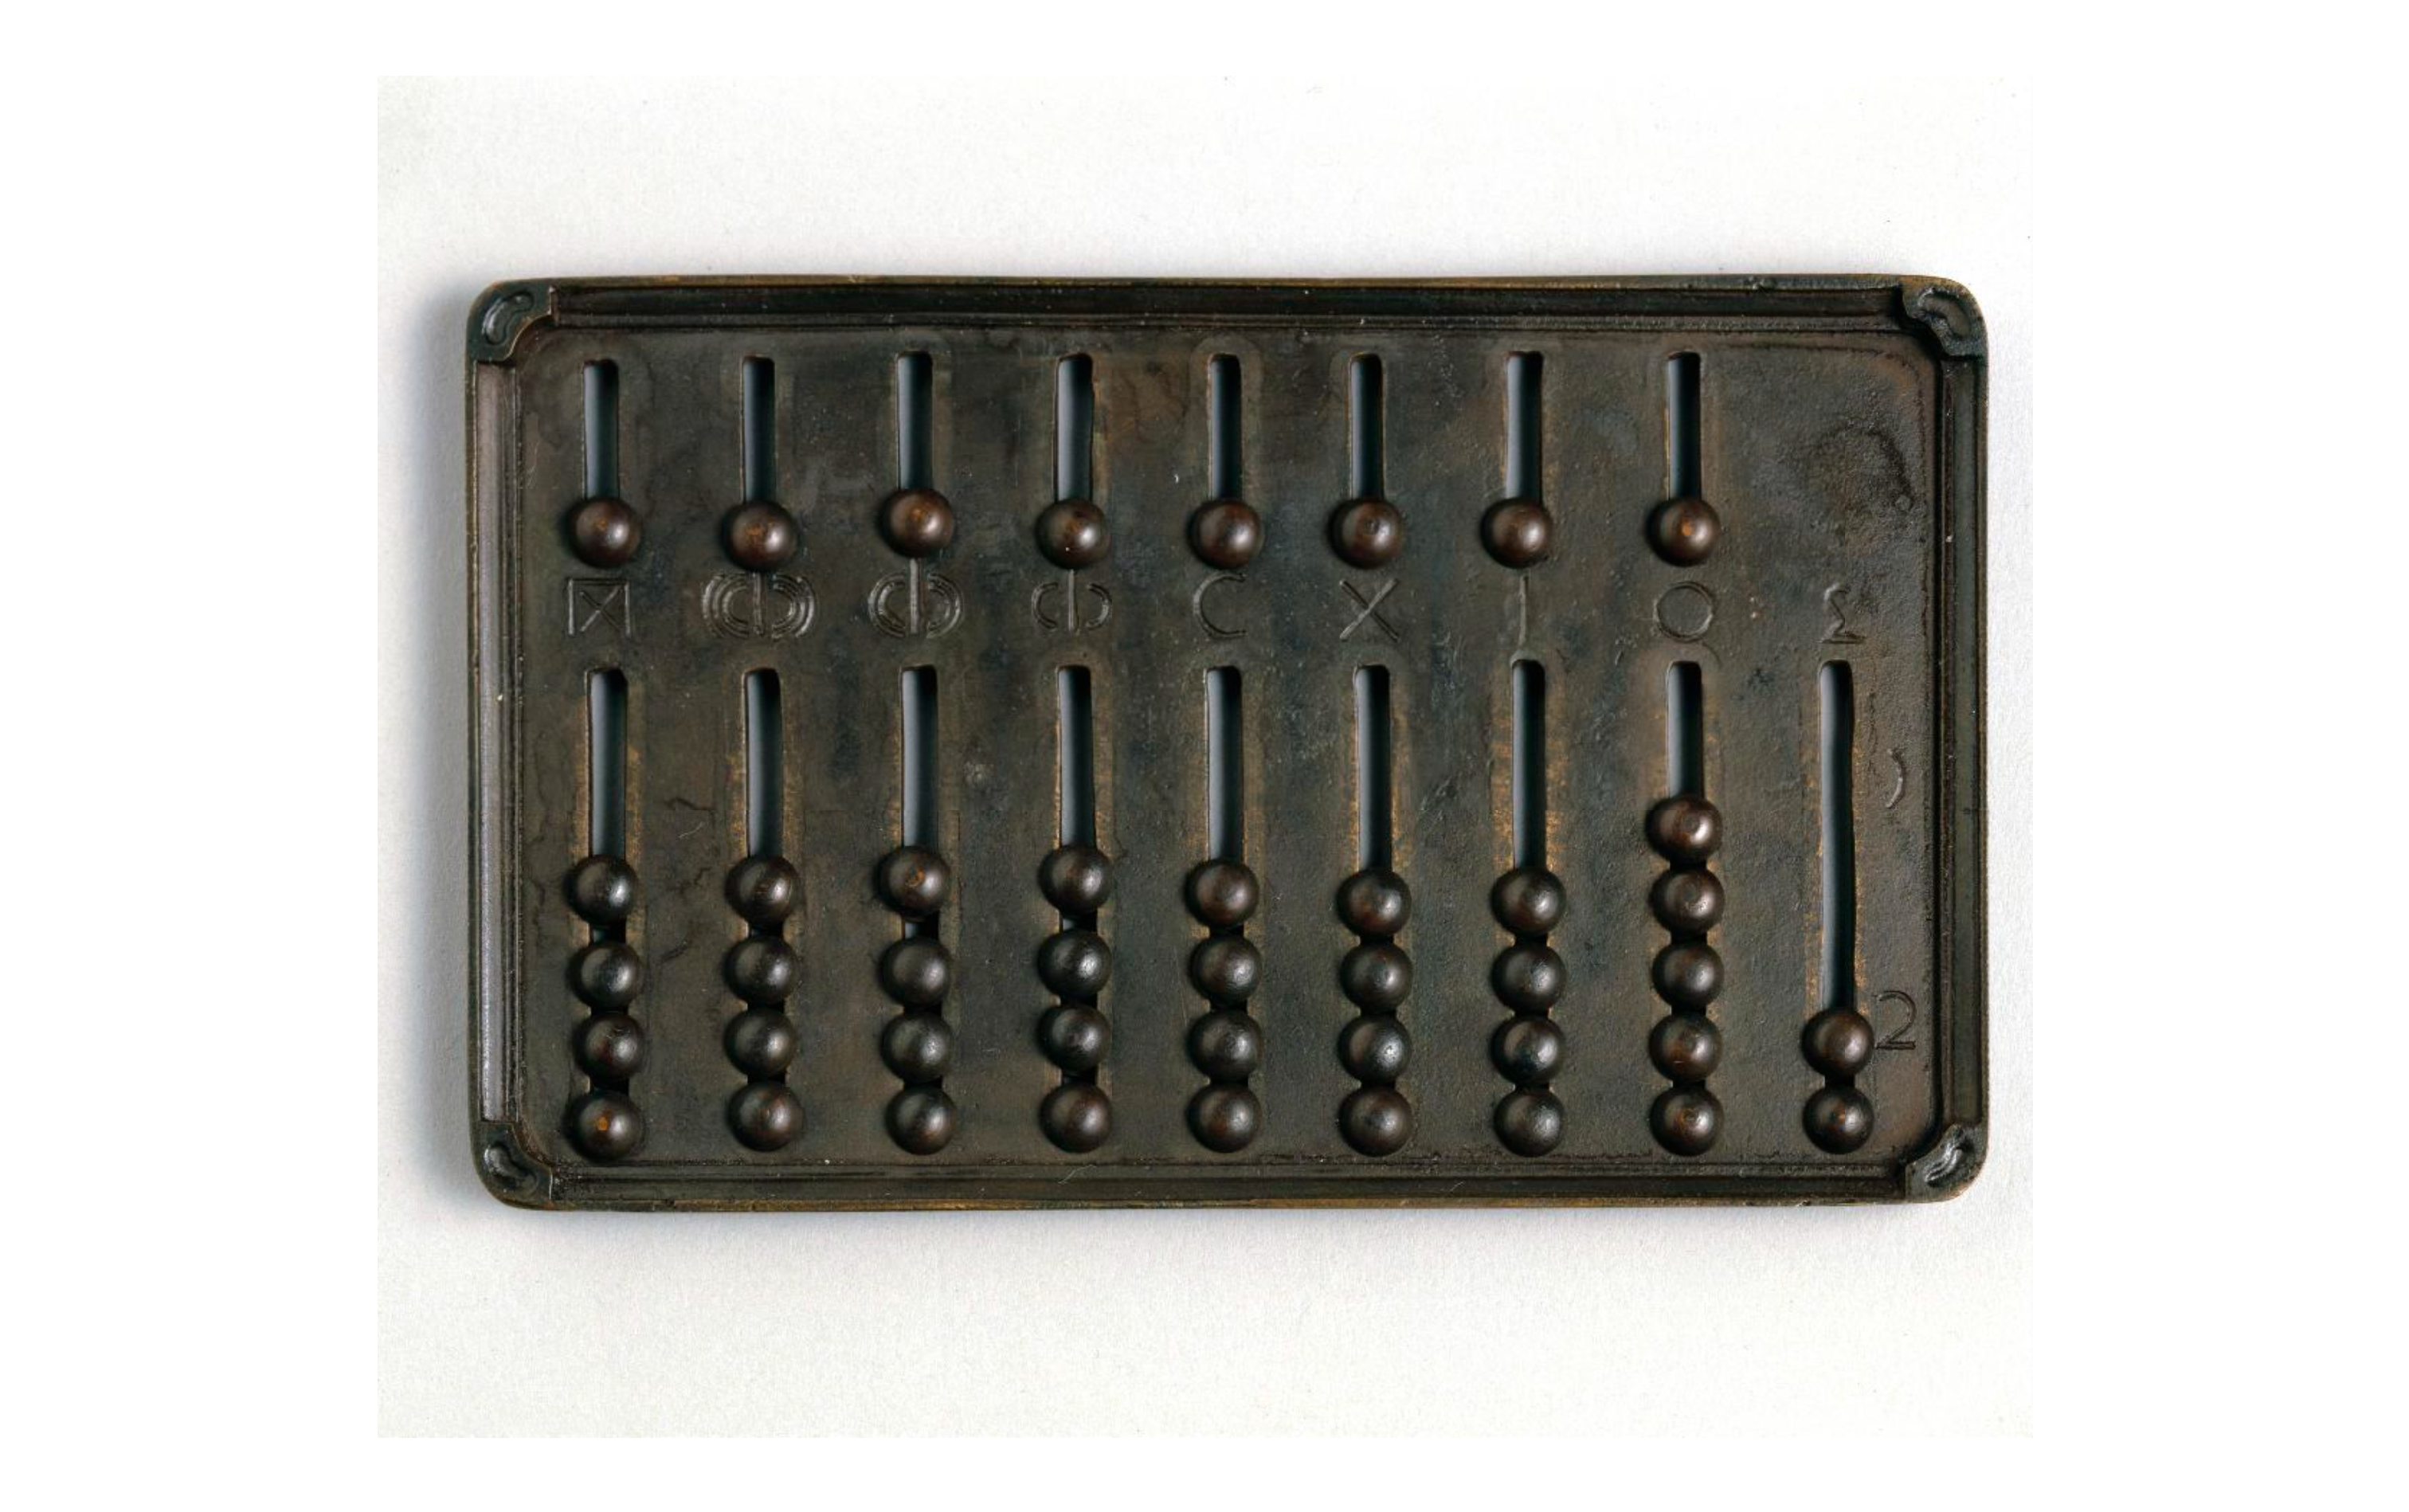
\includegraphics[width=\textwidth]{roman-abacus.png}
    \caption{Abacul roman manual}
    \label{fig:an-ref}
\end{figure}

\subsection*{Gestionarea numerelor întregi și sistemul biquinar}
\quad Secțiunea stângă operează pe baza unui sistem biquinar, sistem în baza 10 care integrează un subsistem în bază 2 pentru valoarea 5. Fiecărui ordin de mărime (unități, zeci, sute etc.) îi sunt alocate două caneluri: în partea superioară una scurtă, dotată cu o singură rivetă (reprezentând 5 unități ale ordinului respectiv), și în partea inferioară una lungă, prevăzută cu patru rivete (fiecare reprezentând o unitate). Pentru reprezentarea unei valori, rivetele sunt glisate astfel încât cele care contribuie la valoarea finală să fie poziționate adiacent axei centrale a instrumentului. De exemplu, reprezentarea cifrei 8 se realizează prin deplasarea rivetei din canelura superioară spre centrul tablei, la care se adaugă deplasarea a trei rivete din canelura inferioară în aceeași direcție. Din punct de vedere funcțional, acest sistem este identic cu cel al sorobanului japonez, similitudine care a generat ipoteze privind un posibil transfer de cunoștințe, cel mai probabil prin intermediul Drumului Mătăsii \cite{stephenson}.

\subsection*{Gestionarea fracțiilor și sistemul duodecimal}
\quad O caracteristică distinctivă a abacului roman o reprezintă cele două caneluri dedicate fracțiilor. Amplasate în extremitatea dreaptă a tablei, sistemul de calcul fracțional utilizează numitorul 12 (fracțiile fiind denumite unciae sau, simplificat, uncii) și este derivat din sistemul monetar și metrologic roman (as-ul și piciorul). \cite{wikipedia}.

Prima coloană destinată calculului de fracții este alocată unciilor și este alcătuită dintr-o canelură superioară cu o singură rivetă, reprezentând 6/12 unități sau o jumătate de uncie, și o canelură inferioară cu cinci rivete, fiecare valorând 1/12 dintr-o unitate, respectiv, o uncie. Această configurație permite reprezentarea valorilor fracționare cuprinse între 1/12 și 11/12.

Cea de-a doua coloană, situată în extrema dreaptă, este considerată cea mai complexă și este intens dezbătută. Consensul științific actual, adoptat de altfel și în prezenta lucrare și fundamentat pe inscripțiile descoperite pe abacurile romane păstrate \cite{wikipedia}, este că: \textbf{riveta în poziția superioară} reprezintă 1/2 dintr-o uncie (respectiv, o semuncia), \textbf{riveta în poziția mediană} reprezintă 1/4 dintr-o uncie (respectiv, un sicilicus) si \textbf{riveta în poziția inferioară} reprezintă 1/6 dintr-o uncie (respectiv, o sextula). Această configurație mixtă permitea efectuarea calculelor financiare și de măsurare într-un mod direct, fără a introduce conversii complicate care ar fi dificile, luând în considerare natura sistemului de numerație roman.

\section*{Utilizare și semnificația istorică}
\quad Utilizarea abacului reprezenta un proces mecanic și vizual, presupunând înțelegerea și memorarea unor algoritmi specifici. Adunarea a două numere mari, de pildă, se realiza prin însumarea succesivă a cifrelor, în ordine descrescătoare a mărimii, iar la depășirea valorii maxime (9) pe o anumită coloană, se efectua un "transport" către ordinul imediat superior, printr-un proces similar algoritmilor de adunare practicați în prezent.

Semnificația istorică a abacului roman este multiplă. În primul rând, instrumentul demonstrează că, deși nu au excelat în matematica teoretică, romanii au fost practicieni desăvârșiți. Inginerii și arhitecții romani au proiectat structuri monumentale fundamentându-și calculele pe asemenea instrumente, cu mult înainte de formalizarea aparatului matematic necesar \cite{ethw}. În al doilea rând, abacul atestă o înțelegere implicită a conceptului de zero; absența oricărei rivete în poziție activă pe o coloană reprezenta, în mod efectiv, valoarea zero pentru respectivul ordin de mărime, constituind o dovadă a faptului că noțiunea de "nimic" era cunoscută și aplicată practic, în ciuda absenței unui simbol dedicat în sistemul de numerație scris.

\section*{Concluzie}
\quad Abacul manual roman este mult mai mult decât o simplă curiozitate arheologică, constituind o dovadă a pragmatismului și ingeniozității romane și o fereastră către modul în care o civilizație antică a rezolvat problemele complexe în ciuda unor limitări științifice majore. Prin designul său portabil, sistemul biquinar pentru numere întregi și coloanele specializate pentru fracții duodecimale, acesta reprezintă o verigă importantă în evoluția dispozitivelor de calcul.

Deși nu este un precursor direct al computerului modern bazat pe silicon, abacul este un precursor notabil al acestuia în linia dezvoltării gândirii computaționale, reamintindu-ne că nevoia de calcule rapide și riguroase este la fel de veche ca însăși civilizația, iar soluțiile găsite de strămoșii noștri sunt adesea de o eficiență și o eleganță deseori subestimate.

\newpage
\begin{thebibliography}{99}

\bibitem{stephenson}
Stephenson, Steve. \textit{The Roman Hand-Abacus}. Toronto Metropolitan University. Disponibil la: \url{https://www.ee.torontomu.ca/~elf/abacus/roman-hand-abacus.html}.

\bibitem{ethw}
Stephenson, Steve. \textit{Ancient Computers}. Engineering and Technology History Wiki (ETHW), 2021. Disponibil la: \url{https://ethw.org/Ancient_Computers}.

\bibitem{knight}
Knight, Stephen. \textit{The Roman Abacus}. Classroom Adventures, 2026. Disponibil la: \url{https://www.classroomadventures.co.uk/post/the-roman-abacus}.

\bibitem{wikipedia}
Wikipedia contributors. \textit{Roman abacus}. Wikipedia, The Free Encyclopedia, 2025. Disponibil la: \url{https://en.wikipedia.org/wiki/Roman_abacus}.

\bibitem{scimuseum}
Science Museum Group. \textit{Roman abacus (replica)}. Science Museum Group Collection. Disponibil la: \url{https://collection.sciencemuseumgroup.org.uk/objects/co59965/roman-abacus}.

\end{thebibliography}

\end{document}